\chapter{Realisierung des Source-To-Source Compilers}
\label{chap:Realisierung}
Gestützt auf das grundsätzliche Wissen über Compiler, die herausgearbeiteten Unterscheidungen von  Xamarin.Forms und Flutter sowie die Differenzen der verwendeten Programmiersprachen  \Csharp und Dart, wird in diesem Kapitel die Realisierung des Source-To-Source Compilers. Um das Projekt mit Roslyn Integration zu implementieren,  bietet sich die \ac{ide} (deutsch Entwicklungsumgebung) Visual Studio 2019 an, da auf dieser Plattform Projekte angelegt werden können, die mit dem Roslyn Compiler interagieren. Die zu entwickelnde Projektmappe, anhand derer der Prototyp validiert werden soll, besteht also aus dem Source to Source Compiler mit Rosyln Integration, der grafischen  Benutzeroberfläche und einer  Xamarin.Forms Anwendung als Testobjekt wobei letzteres erst im nächsten Kapitel eingeführt wird. 

\begin{figure}[!ht]
 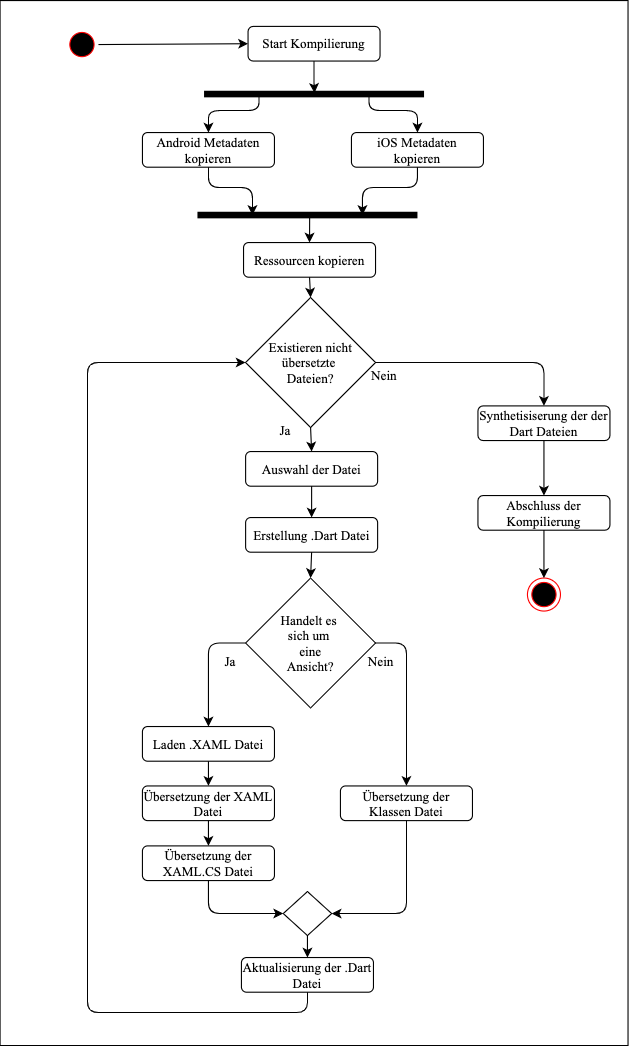
\includegraphics[width=\textwidth,keepaspectratio]{Images/Implementation/Ablauf.png}
 \caption{Aktivitätsdigramm}
 \label{fig:umlablauf}
\end{figure}



\section{Metadaten}


Mit Hilfe von Roslyn konnte der Name des Projektes extrahiert werden.  Dieser Name kann anschließend verwendet werden um ein neues Flutter Projekt zu initialisieren.  

Wie der Quelltext zeigt,  wird dafür ein neues Projekt mit Hilfe der Kommandozeile angelegt.  Damit das Ergebnis nicht von vorherigen Übersetzungsvorgängen beeinträchtigt wird,  auch im Vorhinein überprüft,  ob das Zielverzeichnis existiert und leer ist. 



\section{XAML zu Dart}



\section{C\# zu Dart}


Da sowohl die grafische Benutzeroberfläche als auch der Source-To-Source Compiler mit .Net Technologien realisiert wurden lassen sie sich einfach miteinander kombinieren.  Dafür erhält die  \ac{gui} eine Ahängigkeit auf das \ac{s2s}-Projekt.  



\section{Grafische Benutzeroberfläche}
Die \ac{gui} ist der zentrale Berührungspunkt von Anwendern mit dem Source-To-Source Compiler.  Er spielt soll die notwendigen Eingabe-Möglichkeiten anbieten,  das Ergebnis ausgeben und den Anwender auf mögliche Fehler hinweisen.  Als grafisches Vorbild soll auf das in Kapitel \ref{chap:CompilerEntwurf} entworfene Mockup zurückgegriffen werden.  Für die Erstellung einer grafischen Benutzeroberfläche stehen eine Vielzahl von Technologien mit verschiedenen Vor- und Nachteilen zur Verfügung.  Beispielsweise hätte eine Webseite den Vorteil,  das Anwender keinen Installationsaufwand haben und darüber hinaus auch Plattform-unabhängig auf den Compiler zugreifen können.  Jedoch bringen Webseiten neben dem eigentlichen Entwicklungsaufwand weitere Herausforderungen mit sich,  so haben potentielle Anwender nicht mehr die volle Kontrolle über ihren eigenen Quelltext, wenn sie diesen auf einer Webseite hochladen.  
Aus diesem Grunde,  wird die in dieser Arbeit entworfene Oberfläche eine lokale Anwendung sein,  die von Anwendern lokal installiert werden muss aber im Gegenzug garantiert,  dass niemand Zugriff auf den Source-Code von Anwendern erhält.  Zu diesem Zwecke wird die \ac{gui} mit der Technologie \ac{wpf} realisiert.  Dabei handelt es sich um ein \ac{ui}-Framework des .NET Frameworks welches für die Erstellung von Desktop Anwendungen geeignet ist und mit XAML und \Csharp entwickelt wird.  \footcite[Vgl.][S. 1f]{Wenger2012} Da die Build Tools für Visual Studio nur für Windows Computer ist es auch keine Einschränkung,  dass Anwendungen die mit \ac{wpf} realisiert werden ausschließlich unter diesem Betriebssystem ausführbar sind.

In der Zukunft könnte der Source to Source Compiler auch eine Web-Oberfläche bekommen,  diese hätte die zwei folgenden essentielle Vorteile im Gegensatz zu der aktuellen Implementierung.  Reduktion des Installationsaufwandes - durch den Betrieb über eine Webseite könnte die Installation von der Anzeige entkoppelt werden.  Natürlich wäre eine Client-Server Struktur auch ohne eine Webseite erreichbar,  jedoch haben Webseiten darüber hinaus den zusätzlichen Vorteil,  dass sie Plattform-unabhängig zur Verfügung stehen,  was es zum Beispiel für Xamarin.Forms Entwickelr mit einem Mac OSX Computer erlauben würde ebenfalls von dem Compiler zu profitieren, ohne sich eine Windows Installation vornehmen zu müssen
